\subsubsubsection{Multilayer Perceptron}
\\\\
\indent Ведя разговор о нейронных сетях, нельзя не затронуть сам способ построения подобных моделей. Впервые предложенный Frank Rosenblatt'ом \cite{rosenblatt1961principles}  в 1961 году принцип построения данных моделей, основанный на подобии того, как работает нейрон в мозгу человека, достаточно сильно изменялся, однако идея осталась прежней. По определению <<нейронная сеть>> --- последовательное преобразование признакового пространства. Соответственно формализованный вид данной операции имеет запись:
\begin{equation}
	a(X) = \phi_k(W_k \cdot \ldots \cdot \phi_2(W_2 \cdot \phi_1(W_1 X)))
\end{equation}
Где $W_j: j = \overline{1, k}$ --- некоторая матрица, в общем случае размер ее указать не удается, так как на каждом этапе вычисления получается переход в новое пространство с новой размерностью, $X \in \R^{n \times m}$ --- матрица объект-признак, используемая в качестве входных данных, а $\phi_j : j = \overline{1, k}$ --- используемая на конкретном слое функция активации. Сама же задача, появляющаяся перед исследователем имеет вид:
\begin{equation}
	\frac{1}{m} \sum_{j = 1}^m L(a(x_j | w), y_j) - R(w) \cdot \lambda \to \min_{w}
\end{equation}
Перед нами в общем случае невыпуклая огромная сумма, где $L(\cdot)$ --- функционал потерь, $w = \left\{W_1, \ldots, W_k\right\}$ --- не вектор, а просто набор данных, а $R(\cdot)$ --- функция регуляризации набора весов $w$, необходимая, чтобы уменьшить вероятность переобучения. Соответственно аналитически решение получить невозможно, однако существуют различного рода алгоритмы оптимизации, позволяющие достигать локального/глобального минимума итеративно. В общем случае интуиция, стоящая за достижением минимума, выглядит так:
\begin{equation}
	w^{t + 1} = w^t - \eta^t \cdot \nabla_w \left[L(a(x_j | w), y_j) - R(w) \cdot \lambda\right]
\end{equation}
Наиболее популярными в этой области являются Adam \cite{kingma2014adam}, AdamW \cite{bock2018improvement}, LBFGS \cite{liu1989limited}, а также недавно (2023 год) разработанный Lions \cite{chen2023symbolic}. В настоящем исследовании применяются исключительно LBFGS (для обучения MLP), а также --- в случаях, когда LBFGS дает неудовлетворительный результат --- AdamW как наиболее распространенный (универсальный) его заменитель.

Сама идея алгоритма обучения завязана на применение теоремы о дифференцировании сложной функции, так как $a(\cdot)$ именно ей и является. Таким образом, для вычисления такого количества производных используется алгоритм под названием BackPropagation \cite{linnainmaa1970representation}. Принцип его работы заключается в дифференцировании графа вычислений, схематично представляющего исходную нейронную сеть. В формальном виде:
\begin{equation}
	\frac{\partial L}{\partial w} = \left. \frac{\partial f_1}{\partial w} \right\rvert_w \left. \frac{\partial f_2}{\partial f_1} \right\rvert_{f_1(w)} \cdot \ldots \cdot \left. \frac{\partial f_k}{\partial f_{k - 1}} \right\rvert_{f_{k - 1}(\cdot)} \left. \frac{\partial L}{\partial f_k} \right\rvert_{f_k\left(f_{k - 1}(\cdot)\right)} = \nabla_w L
\end{equation}
Интересно отметить, что существует теорема, гласящая, что, имея однослойную нейронную сеть, можно с любой точностью приблизить абсолютно любую непрерывную функцию многих переменных \cite{cybenko1989approximation}.

В качестве примера рассматриваем способность к прогнозированию на один рабочий день биржи модели MLP для цен акций открытия компании Ford, начиная с даты выхода компании на IPO, а заканчивая 13/12/2022 годом.
\begin{figure}[H]
	\centering
	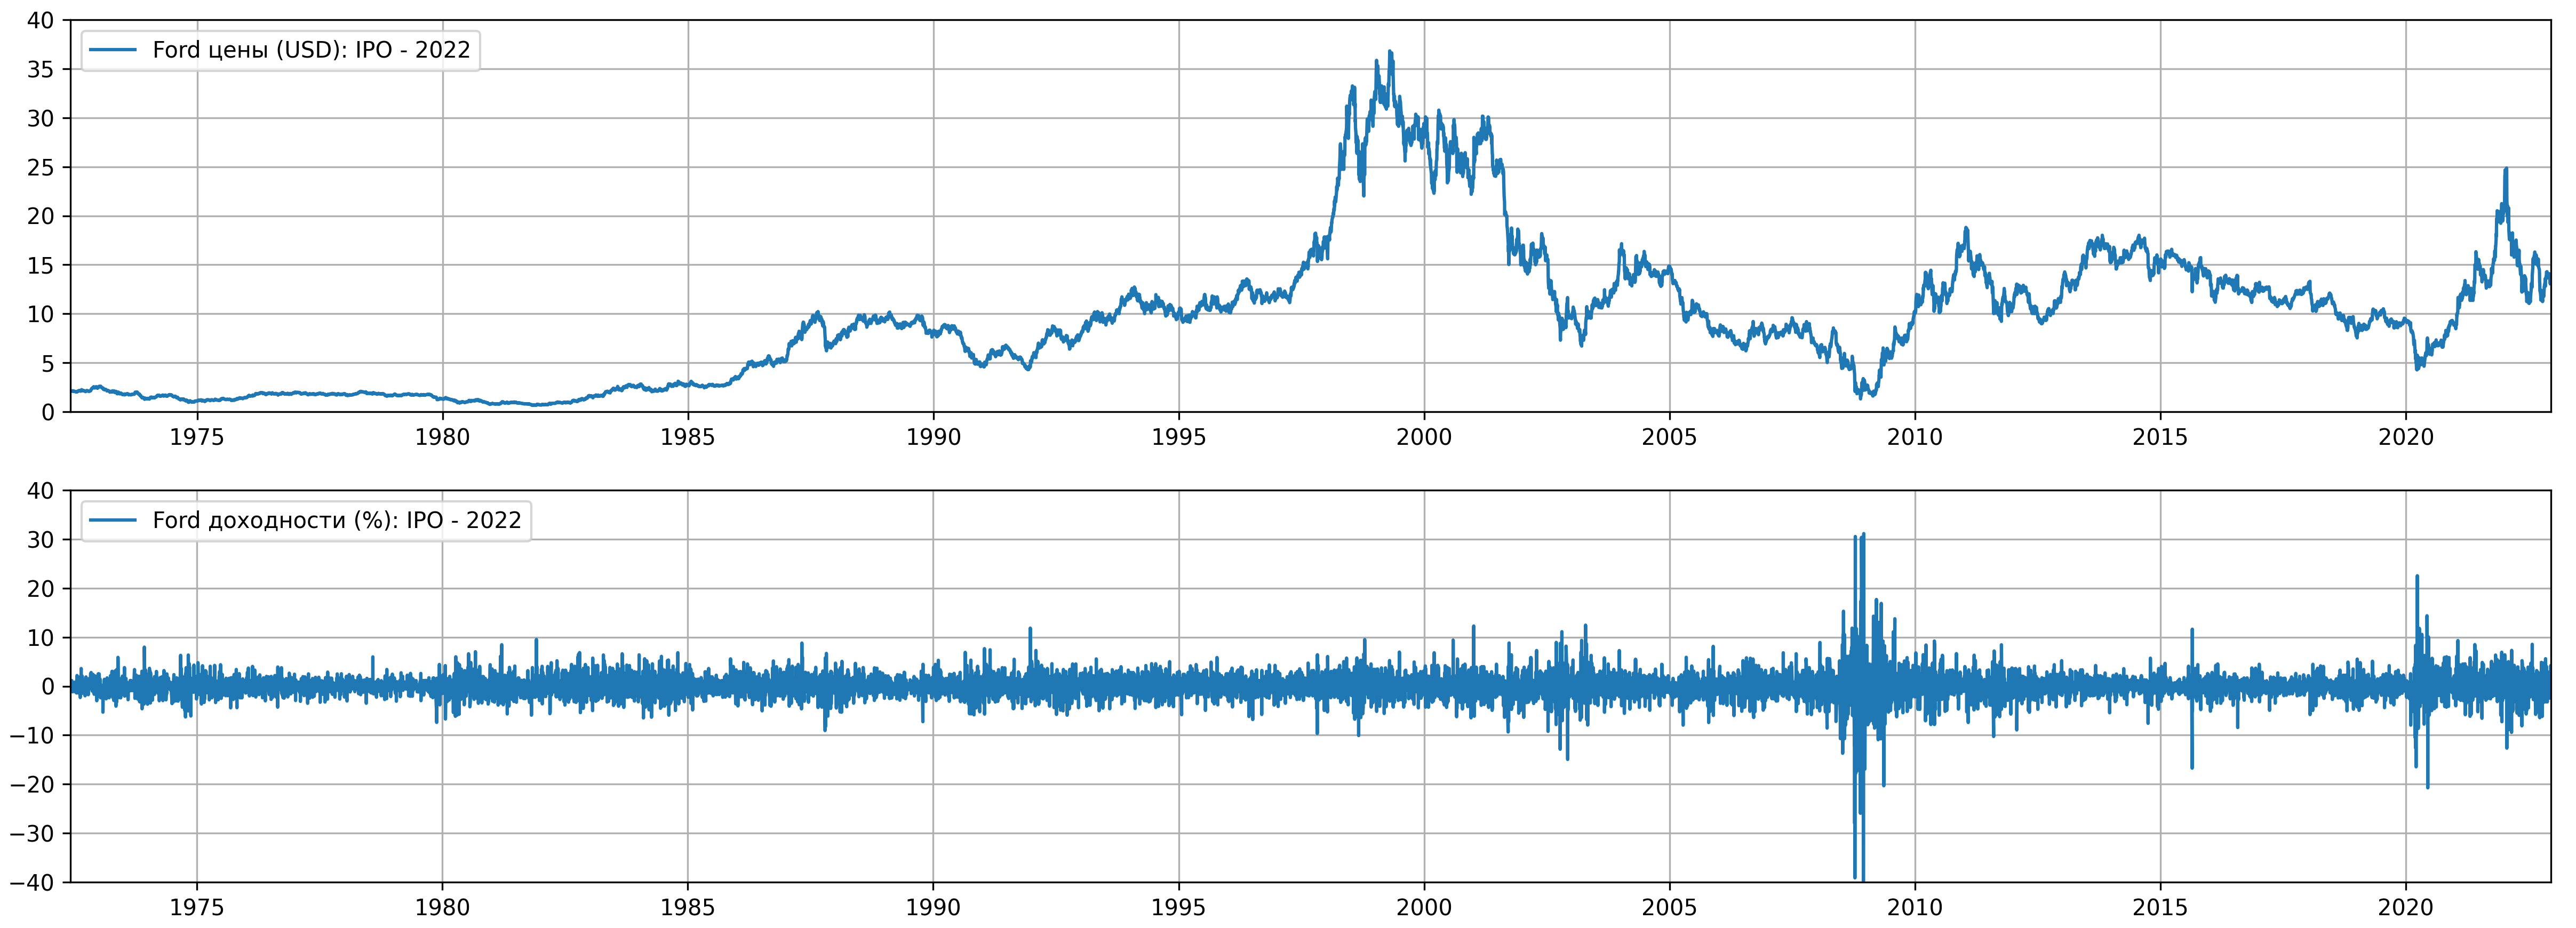
\includegraphics[width=17cm]{returns pictures/ford_prices_returns.png}
	\caption{График цены открытия и доходности Ford (IPO --- 2022)}
	\label{fig::ford_prices_returns}
\end{figure}
Далее смотрим на показатели функции потерь для обучающей выборки и валидационной по мере обучения самой модели. В качестве функции потерь в данном случае используется уже ранее обсуждавшаяся MSE, а в качестве метрики выбрана WAPE (Weighted Average Percentage Error):
\begin{figure}[H]
	\centering
	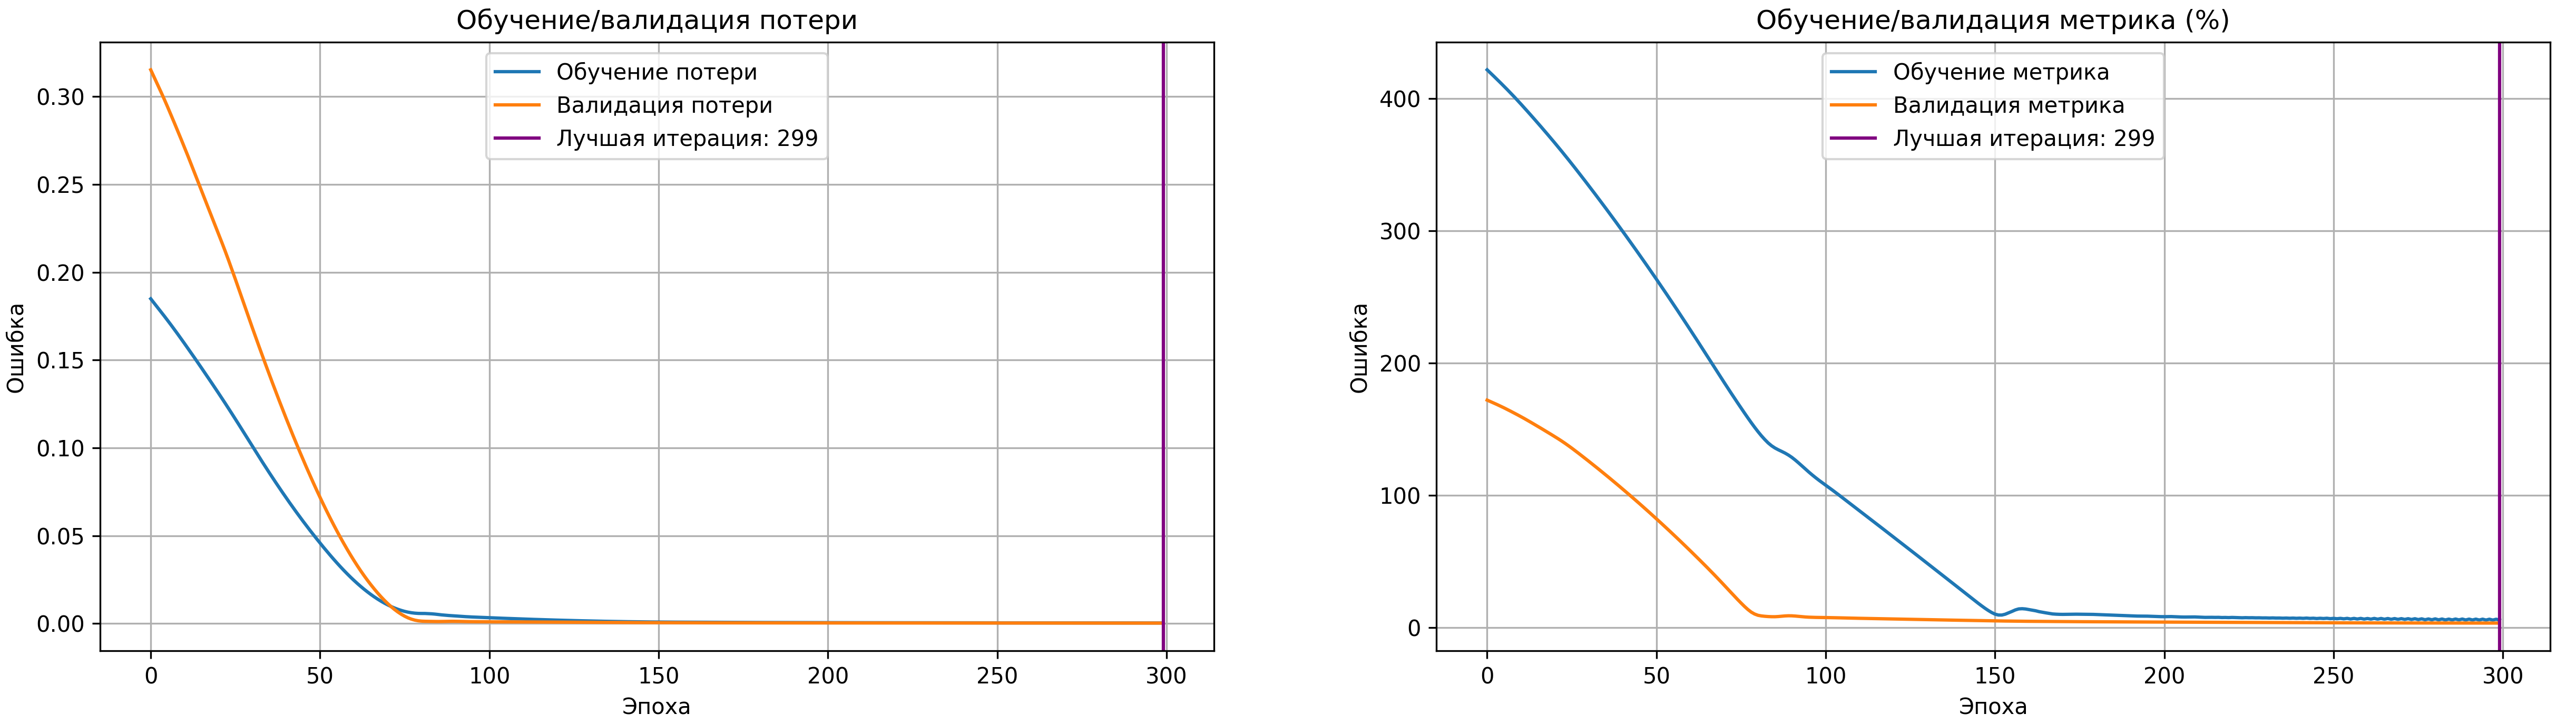
\includegraphics[width=17cm]{nn/mlp/ford_train_val_results.png}
	\caption{График MSE для модели MLP}
	\label{fig::ford_train_val_results}
\end{figure}
Но также интересно, как менялось значение лучшей валидационной метрики, ведь именно она является критерием сохранения весов модели. Принцип прост: если меньше максимального, сохраняй модель. Более подробно: после прохода по всей обучающей выборке (то есть после прохождения <<эпохи>>) происходит валидационный цикл, во время которого вычисляется WAPE. Если WAPE на шаге $t$ меньше, чем WAPE на шаге $t - 1$, то веса, полученные в модели на момент $t$ сохраняются в отдельный файл. После чего перед началом тестового цикла, во время которого вычисляется WAPE для тестовых данных, происходит <<загрузка>> в модель полученных на <<лучшей>> итерации весов, исходя из которых далее получается финальное значение выбранной метрики --- в нашем случае, WAPE.
\begin{figure}[H]
	\centering
	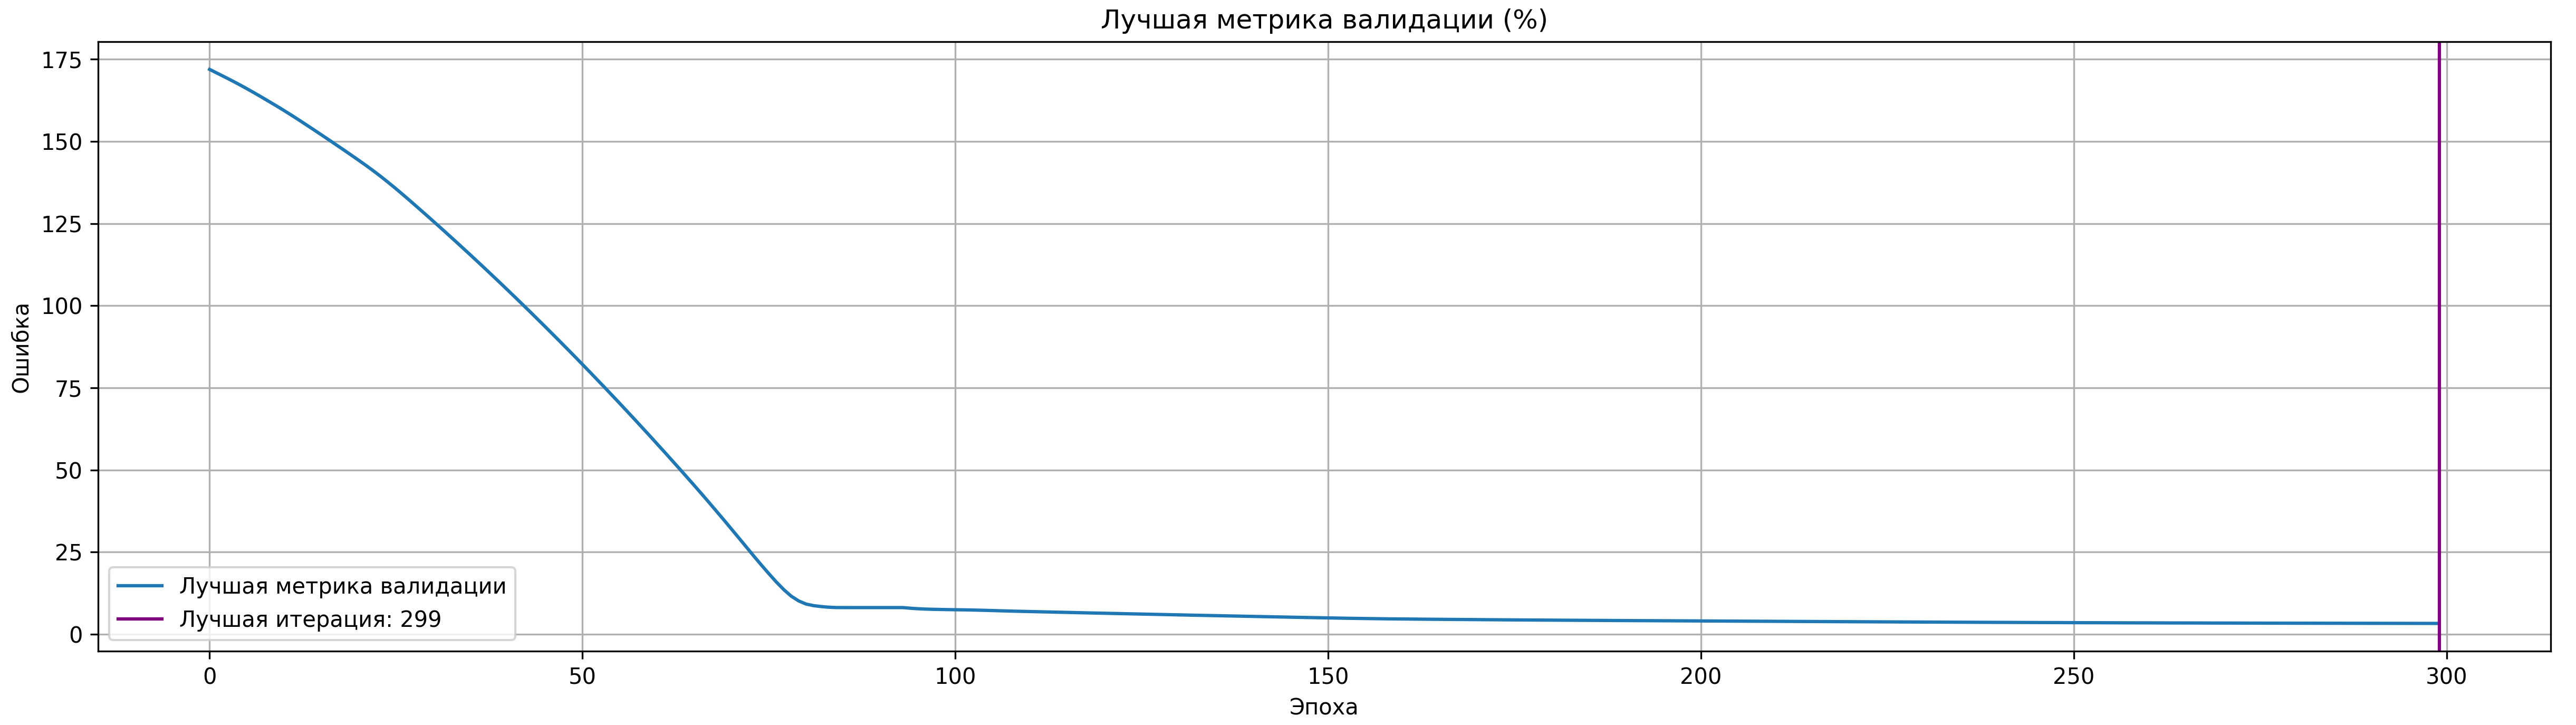
\includegraphics[width=17cm]{nn/mlp/ford_best_metric_results.png}
	\caption{График изменения лучшей валидационной метрики: WAPE$(y, \hat{y}) = \sum_{t = 1}^n |y_t - \hat{y}_t| / \sum_{t = 1}^n |y_t|$}
	\label{fig::ford_train_best_metric_results}
\end{figure}
Финальным этапом является построение прогноза и подсчета получившейся ошибки в терминах процентного отклонения WAPE и аналогично ранее указанной RMSE.
\begin{figure}[H]
	\centering
	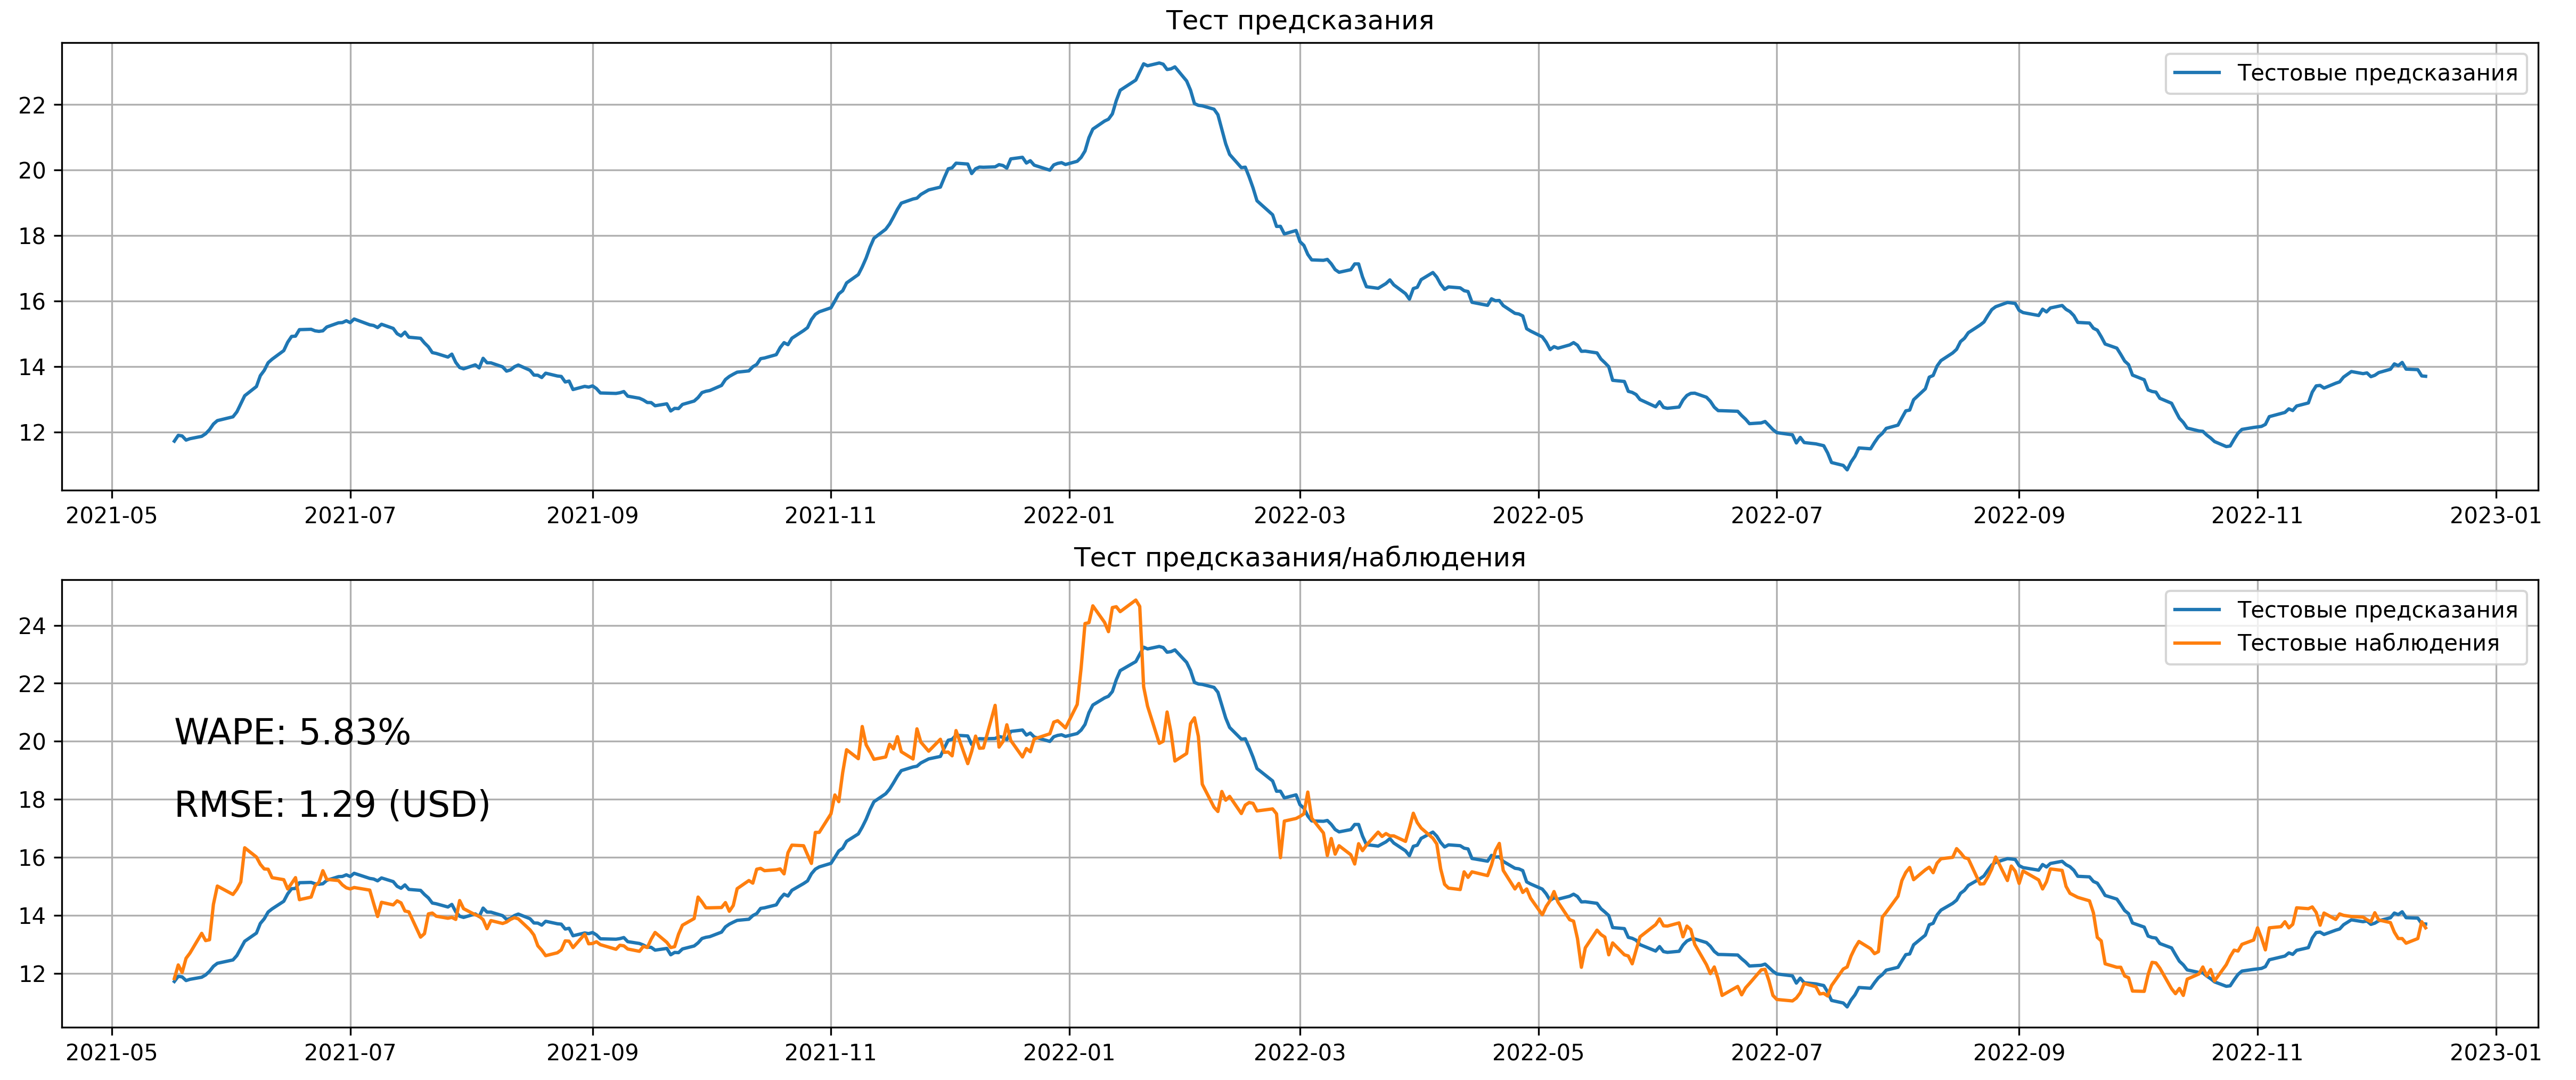
\includegraphics[width=17cm]{nn/mlp/ford_test_results.png}
	\caption{График реальных и предсказанных значений цен акций Ford (USD)}
	\label{fig::ford_test_results}
\end{figure}
Очевидно, что методика неплохо работает, так как полученная метрика без наличия тюнинга (подбора гиперпараметров) составляет $\pm 1.29$ USD, что достаточно мало, но существенно в случае большого количества акций, с которыми совершается операция. Нельзя сказать, что полученный результат является неприменимым к жизненным ситуациям, хотя без оговорок не обойтись: ошибка слишком велика в денежном эквиваленте, таким образом, лучше опираться на выводы полученной модели при оперировании небольшой суммой денег, так как сама по себе ошибка растет прямо пропорционально сумме операции. Однако остается провести аналогичное исследование для доходностей, чтобы в полной мере понять способность модели к прогнозированию. Так как обучение модели на ценах, исходя из визуального анализа графика, кажется более естественным по причине наличия некоторого тренда, нежели аналогичное действие по отношению к доходностям в условиях их волатильности и резких изменений. Другими словами, доходности более похожи на звуковую дорожку, чем на некоторый процесс.
\begin{figure}[H]
	\centering
	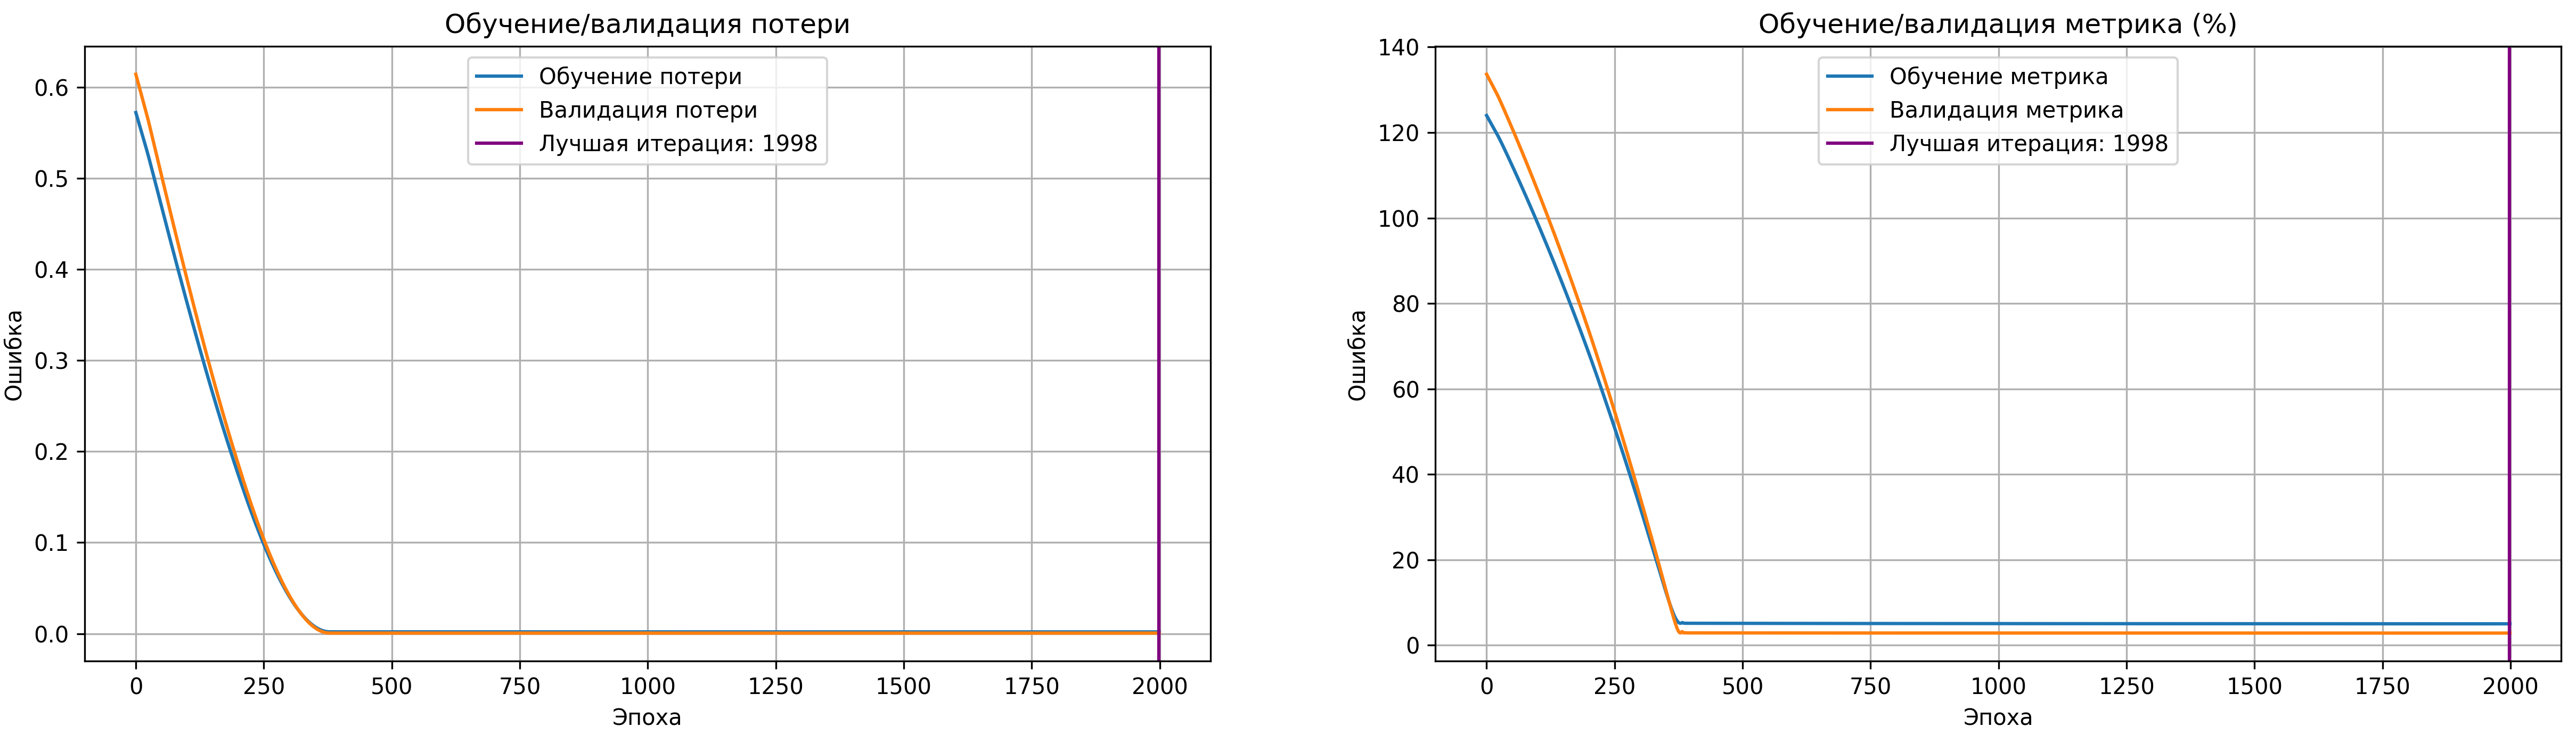
\includegraphics[width=17cm]{nn/mlp/ford_train_val_returns_results.png}
	\caption{График MSE для модели MLP (доходности \%)}
	\label{fig::ford_train_val_returns_results}
\end{figure}
Поведение достаточно схожее с моделью на ценах, то есть обучение выполняется достаточно успешно. Однако пока что это ничего не говорит о самом поведении модели на тестовой выборке, ведь данная кривая символизирует лишь успешную сходимость к минимуму. То есть даже, если ошибка мала, результат может быть неудовлетворительным, из-за необходимости обоснования поведения обученной модели, исходя из логической составляющей, прикладываемой к реальности. Иными словами, полученные результаты должны согласовываться с реальностью, даже если показатель ошибки минимален.
\begin{figure}[H]
	\centering
	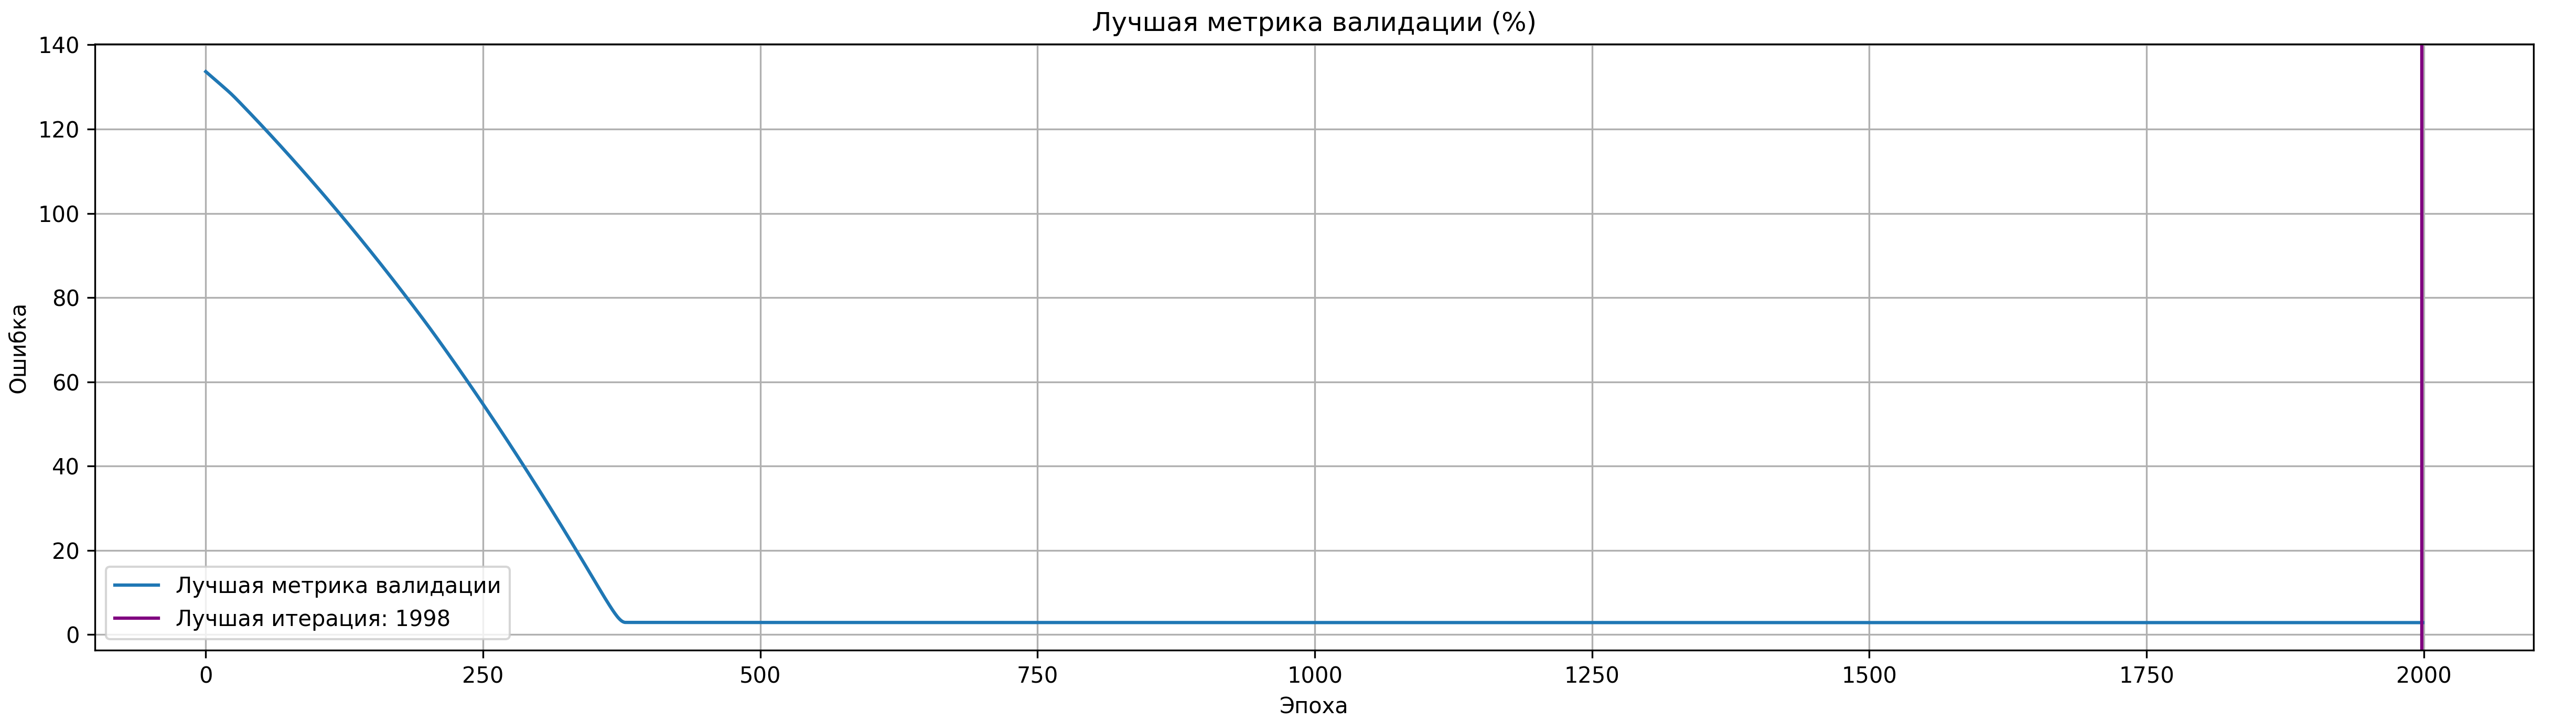
\includegraphics[width=17cm]{nn/mlp/ford_best_metric_returns_results.png}
	\caption{График изменения лучшей валидационной метрики: WAPE$(y, \hat{y}) = \sum_{t = 1}^n |y_t - \hat{y}_t| / \sum_{t = 1}^n |y_t|$ (доходности \%)}
	\label{fig::ford_best_metric_returns_results}
\end{figure}
Видим, что ошибка по мере продвижения по эпохам ведет себя <<хорошо>>, то есть достаточно стремительно убывает, однако на 375 итерации выходит на плато. Соответственно, изменение ошибки на данном плато достаточно мало, следовательно, необходимо либо динамически изменять скорость обучения (выше описанный параметр $\lambda$, он же learning rate --- далее lr) или изначально брать lr больше, чтобы <<проскочить>> достигнутый минимум. Дополнительный вариант действий, который может привести к улучшению результата --- использование либо более сложной архитектуры, либо более простой, чтобы видоизменить поверхность функции потерь, по которой <<скатывается>> ее градиент. Теперь, опираясь на сказанное ранее, смотрим на предсказания для тестовой выборки, из которых далее делаем вывод о качестве работы обученной модели.
\begin{figure}[H]
	\centering
	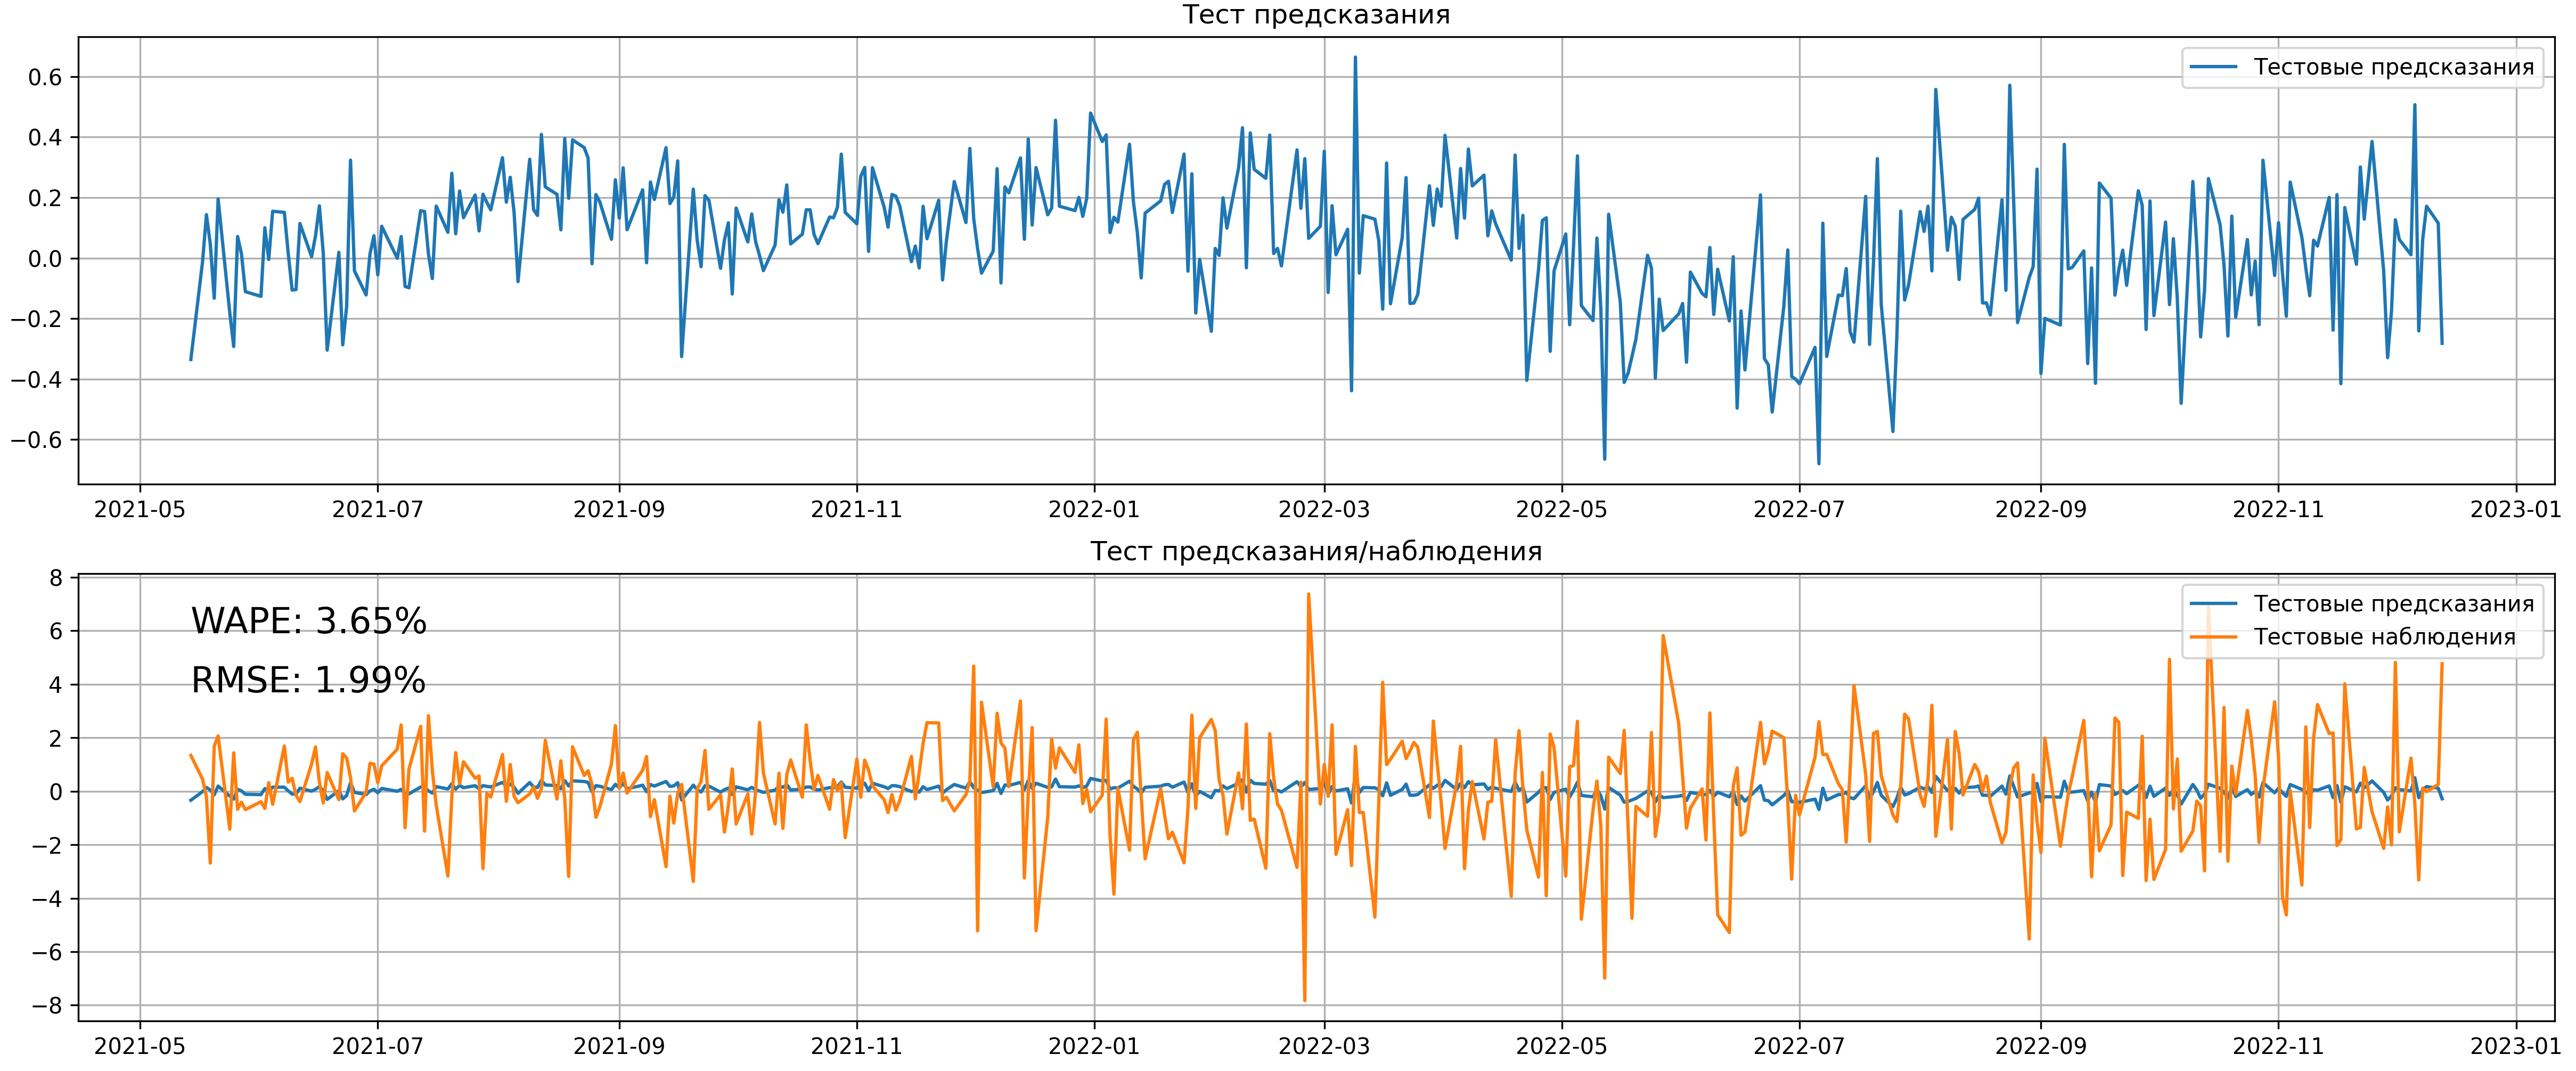
\includegraphics[width=17cm]{nn/mlp/ford_test_returns_results.png}
	\caption{График реальных и предсказанных доходностей акций Ford (\%)}
	\label{fig::ford_test_returns_results}
\end{figure}
Очевидно, что полученный результат, хотя и полученная ошибка мала, не является удовлетворительным и применимым к реальности, так как, основываясь на метрике RMSE, имеем отклонение $\pm 1.99\%$, что заметно больше, чем средняя предсказанная величина. Таким образом, настоящая модель не только не может быть применена к реальности, но и способна ввести в заблуждение относительно ответа на вопрос <<Buy, Hold or Sell>>. 

Также замечаем, что поведение предсказанных показателей как будто сдвинуто немного вперед. То есть в реальности уже было, а в прогнозе --- только будет. Подобное возможно по трем причинам: малая мощность модели, непригодность модели, особенность рассматриваемых данных. Значит, нельзя делать поспешные выводы о качестве самой модели, ведь анализ велся только для одной компании. Финальный ответ о пригодности той или иной модели рассматривается в заключении настоящего исследования. Однако текущая модель включается в финальную таблицу как способная к прогнозированию как цен, так и доходностей.